
\renewcommand{\caseUseShortName}{cancelarOrdenProduccion} %cammelCase name

\renewcommand{\caseUseCreated}{05/03/2020} %Fecha creación
\renewcommand{\caseUseModified}{05/03/2020} %Fecha modificación
\renewcommand{\caseUseName}{\CUcancelarOrdenProduccion - Cancelar orden de producción} %{\CUcammelCase - Title}

\renewcommand{\caseUseSummary}{Este caso de uso permite a un administrador de ZMGestion cancelar una orden de producción.} %Resumen
\renewcommand{\caseUsePeople}{Administradores: quiere cancelar una orden de producción existente.} %Actor: Meta
\renewcommand{\caseUsePreconditions}{
	\caseUseRow{Haber realizado con éxito el CU92\ (Buscar avanzado órdenes de producción).}
}
\renewcommand{\caseUsePostconditions}{
	\caseUseRow{Ninguna.} %Postcondiciones
}
\renewcommand{\caseUseScene}{ %Escenario principal
    \addCaseUseStep{El administrador selecciona una orden de producción que desea cancelar.}
    \addCaseUseStep{ZMGestion ejecuta el \CUcancelarLineaOrdenProduccion\ (Cancelar línea orden de producción) para cada línea de la orden de producción que se encuentre `Pendiente de producción' o `En producción'.}
}
\renewcommand{\alternativeCaseUse}{ %Flujos alternativos
	\newAlternative{A1: La orden de producción seleccionada no se encuentra en estado `Pendiente' o `En producción'.}{1} %Flujo alternativo A1.
	\caseUseRow{La secuencia A1 comienza luego del punto 1 del escenario principal.} %¡Indicar número paso!
    \alternativeRow{ZMGestion muestra un mensaje de error indicando que la orden de producción no puede cancelarse.}
    \caseUseRow{El escenario vuelve al punto 1.}
    \caseUseRow{}
}

%\item Caso de uso \caseUseName
\renewcommand*{\arraystretch}{1.3}
\begin{longtable}[c]{|>{\raggedright}p{0.3\textwidth} | >{\raggedright}p{0.2\textwidth} | p{0.5\textwidth} |}
\caption{\hyperref[sec:listadoCasoUso]{\caseUseName}}
\label{tabla:\caseUseShortName}\\
\hline
\rowcolor{tableCaseUseBackground}

\multicolumn{3}{|l|}{\textcolor{tableCaseUseFontColor}{Descripción textual del caso de uso: \caseUseName}} \\ \hline

Fecha de Creación: & \multicolumn{2}{L{\secondColumnWidth}|}{\caseUseCreated}\\ \hline

Fecha de Modificación: & \multicolumn{2}{L{\secondColumnWidth}|}{\caseUseModified} \\ \hline

Versión: & \multicolumn{2}{L{\secondColumnWidth}|}{1} \\ \hline

Resumen: & \multicolumn{2}{L{\secondColumnWidth}|}{\caseUseSummary} \\ \hline

Personas involucradas y metas: & \multicolumn{2}{L{\secondColumnWidth}|}{\caseUsePeople} \\ \hline

Precondiciones: \caseUsePreconditions \hline

Postcondiciones: \caseUsePostconditions \hline

Escenario principal: \caseUseScene \hline

Flujos alternativos: \alternativeCaseUse \hline

Requisitos de interfaz de usuario: \caseUseRequirementsGUI \hline
\multirow{3}{*}{Requisitos funcionales:}  & Tiempo de respuesta: & \caseUseResponseTime \\ \cline{2-3} 
& Concurrencia: & \caseUseConcurrence \\ \cline{2-3} 
& Disponibilidad: & \caseUseAvailability \\ \hline
\end{longtable}

\setcounter{rownumbers}{0}

\renewcommand{\alternativeCaseUse}{
	\caseUseRow{No existen flujos alternativos.}
}

%DIAGRAMA DE ACTIVIDAD
%\lineabreak[0]
\begin{figure}[H]
    \centering
    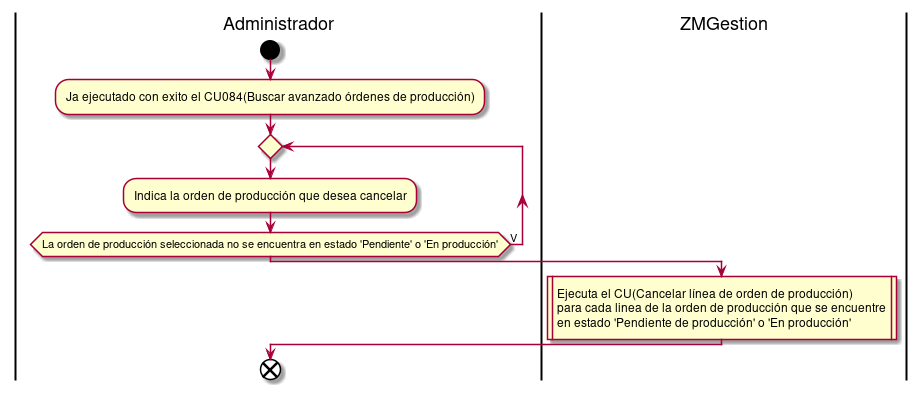
\includegraphics[width=\textwidth,height=0.95\textheight,keepaspectratio]{DiagramasActividad/DiagramaDeActividad/cancelarOrdenProduccion}
    \caption{CU94 - Cancelar orden de producción}
\label{fig:cancelarOrdenProduccion}
\end{figure}